\documentclass{article}
\usepackage[utf8]{inputenc}
\usepackage[spanish]{babel}
\usepackage[legalpaper, portrait, margin=1in]{geometry}
\usepackage{setspace}
\onehalfspacing
\usepackage{parskip}
\setlength{\parindent}{0cm}
\usepackage{enumitem}
\setlist{nosep}
\usepackage{hyperref}
\usepackage{graphicx}

\hypersetup{
  	colorlinks,
	citecolor=black,
	filecolor=black,
	linkcolor=black,
	urlcolor=black
}
\title{%
  Olympus DAO Manifiesto \\
  \large Una DAO funcional para projectos Open Source de cryptomonedas }
\author{
  Berrueta, Enrique\\
  \texttt{eabz@polispay.org}
  \and
  Bustos, Ricardo\\
  \texttt{eros@polispay.org}
}
\date{Junio 2020}

\begin{document}

\maketitle

	\begin{abstract}
	Una DAO es una ``Organizacion Autonoma y Decentralizada`` o una institución sin una autoridad central que puede ser governada por un grupo de miembros autorizados y elegidos por una comunidad mayor. A lo largo de los años, muchas DAO e intentos de governanza se han intentado desde el nacimiento de las cryptomonedas. Desde Dash hasta "The DAO" de Ethereum, todos estas organizaciones han tenido varios problemas, desde la falta de organización hasta caer un en una centralización. Después de reflexionarlo, hemos llegado a proponer una nueva solución para proponer un modelo funcional de una DAO, que no sólo será decentralizada sino tambien organizada e inclusiva.
	\end{abstract}

\newpage

\tableofcontents


\newpage

\section{Estructura}

La DAO se basará en cinco pilares fundamentales, sobre los cuales habrá una persona encargada elegida por la comunidad para cada área:

\begin{itemize}
  \item Tecnología.
  \item Comunidad.
  \item Negocios.
  \item Adopción.
  \item Marketing.
\end{itemize}

\begin{figure}[h]
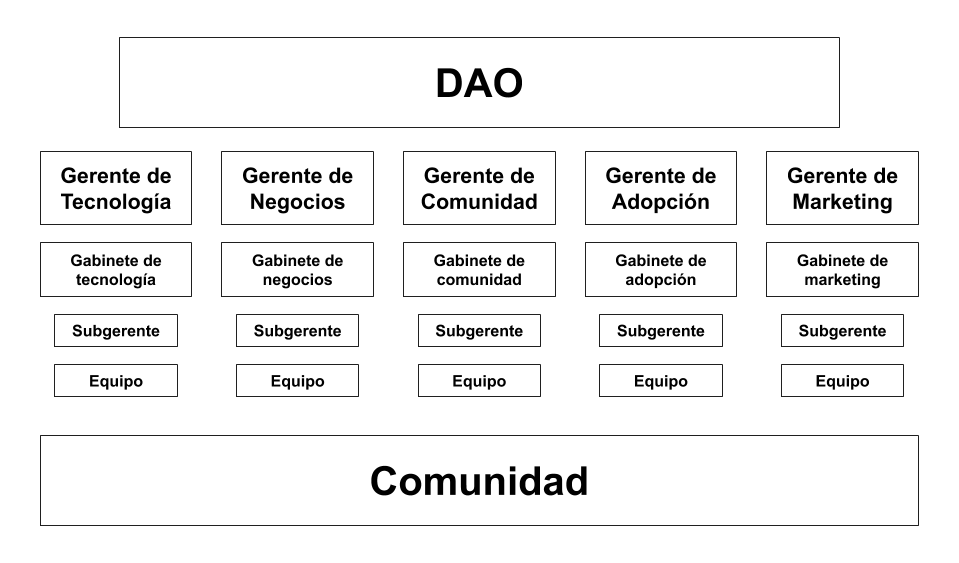
\includegraphics[scale=0.4]{img/dao_structure_es.png}
\centering
\caption{Modelo básico de la estructura de la DAO}
\end{figure}

Cada persona a cargo, que de ahora en adelante se le llamará ``Gerentes`` será elegible dependiendo de su prestigio en la comunidad. Esa persona presentará una propuesta a la comunidad donde detallará su propuesta de trabajo para el cyclo de mando, que durará un año.

En su propuesta los gerentes deberan delinear los siguientes puntos:

\begin{itemize}
  \item Propuestas de mejora.
  \item Miembros de su equipo (Gabinete).
  \item Estrategias que emplearan para lograr sus propuestas.
  \item Razones por las que deberían de votar por él.
  \item Plan de trabajo detallado fon tiempos establecidos.
\end{itemize}

Los gerentes serán elegibles para reelección las veces que ellos quieran siempre y cuando la comunidad este deacuerdso con ellos.

\section{Llaves}

Puesto que la DAO se refiere a un ecosystema en torno a las cryptomonedas, todo lo relacionado con los votos y mecanismos de toma de decisiones se hace usando las Llaves de la DAO. Estas Llaves son aseguradas por los gerentes y el accesso es otorgado/eliminado mediante los ciclos de votacion o la ejecución de un mecanismo de defensa.

Estas llaves se cambiarán cada cyclo de votos o si algun mecanismo de seguridad se activa. Esta llave será la receptora de los fondos otorgados para cada área y se usará para desbloquear los fondos (junto con los otros gerentes) del fondo para propuestas de la comunidad y sobre-cargos de las demás áreas.

\section{Plataforma}

La plataforma para interactuar, votar y proponer en la DAO es la blockchain de Olympus.

Cualquier usuario pódrá vertificar la información con un nodo de Olympus.

La Cartera de Olympus es la plataforma principal que los usuarios tendrán para verificar la información de la DAO.

\section{Tesoro}

Para que la DAO funcione apropiadamente como una organización es completamente necesario tener fondos. Esto no es posible basandose únicamente en donaciones, es por eso que proponemos un modelo de obtención de fondos que garantiza una distribución equitativa para cada área.

El 20\% de la emisión total de monedas será bloqueado para la DAO.

Estos fondos se distribuirán en tres categorías:

\begin{itemize}
  \item 10\% para las áreas de la DAO.
  \item 5\% para las propuestas de la comunidad.
  \item 5\% bloqueados para los sobre-cargos de cada área.
\end{itemize}

El presupuesto de las áreas se distribuirá en las siguientes proporciones:

\begin{itemize}
  \item 30\% Tecnología.
  \item 10\% Comunidad.
  \item 20\% Negocios.
  \item 20\% Marketing.
  \item 20\% Adopción.
\end{itemize}

El 5\% para las propuestas de la comunidad será distribuido basado en la decisión de los gerentes. Ellos decidirán cuando una propuesta debe de ser fondeada.

El 5\% para los sobre-cargois de un área serán usados de acuerdo a la decisión de los gerentes para incrementar el presupuesto de algún área en algún periodo especifico.

Estos fondos serán depositados cada mes a las llaves de cada uno de los gerentes de las áreas.   

Los fondos para las propuestas de la comunidad y los sobre-cargos serán depositados a una llave multi-firma para asegurar que solamente 3 de 5 gerentes puedan sacar esos fondos.

Las propuestas de la comunidad deben detallar:

\begin{itemize}
  \item Cantidad de dinero solicitado.
  \item Plan de trabajo.
  \item Presupuesto detallado con costos.
\end{itemize}

\section{Ciclos}

La funcionalidad de la DAO se fundamenta en ciclos de tiempo. Hay tres cyclos principales que involucran deciciones en diferentes momentos.

\subsection{Ciclo de Votos}

El cyclo de votos empieza cada año el día 20 de Enero. Este proceso toma alrededor de 2 or 3 semanas. La idea es tener un proceso de campaña electoral en el que los gerentes antiguos y los nuevos que quieran involucrarse en la dirección de la DAO deberán presentar sus propuestas y planes de trabajo para ser calificados.

El ciclo tiene cuatro fases:

\begin{itemize}
  \item Postulación de candidatos.
  \item Propuestas de candidatos.
  \item Preparación de las elecciones.
  \item Votación.
\end{itemize}

\subsection{Ciclo de presupuestos}

Una vez que los miembros de la DAO son elegidos, ellos deben de crear un presupuesto por medio del cuál operarán los siguientes tres meses. Este presupuesto deberá de ser presentado por el Gerente de Negocios cada tres meses incluyendo los gastos reales para otorgarle a la comunidad información transparente.

\subsection{Cyclo de reportes}

Además del ciclo de presupuestos, cada gerente deberá de entragar un reporte dentro de su propia área donde exponga los logros del trabajo de los tres meses a los demás gerentes y a la comunidad.

Si un gerente no sube sus reportes a la red, su llave quedará automaticamente eliminada.

\section{Áreas}

\subsection{Tecnología}

El gerente a cargo del área de tecnología será responsable de contratar y entrenar desarrolladores que sigan el plan de trabajo técnico de la DAO.

El gerente tendrá las siguientes responsabilidades:

\begin{itemize}
  \item Desarrollo técnico de la cryptomoneda.
  \item Desarrollo de casos de uso.
  \item Librerías de terceros.
  \item Documentación y mantenimiento.
\end{itemize}

Junto con el gerente de la comunidad, esta encargado de la funcionalidad y documentación de los siguientes servicios:

\begin{itemize}
  \item Exploradores de bloques officiales.
  \item Paginas web.
  \item Guías.
  \item Foros.
  \item Recursos internos.
\end{itemize}

\subsection{Comunidad}

El gerente encargado de la comunida tendrá la responsabilidad de la integridad y exactitud de la información en los distintos canales, asì como resolver los problemas técnicos de los miembros de la comunidad.

El gerente tendrá las siguientes responsabilidades:

\begin{itemize}
  \item Comunicación y redes sociales.
  \item Documentación mantenimiento.
  \item Soporte tecnico y buenas prácticas de seguridad.
  \item Correcto uso de la marca y diseños.
\end{itemize}

Junto con el gerente de la tecnología, esta encargado de la funcionalidad y documentación de los siguientes servicios:

\begin{itemize}
  \item Exploradores de bloques officiales.
  \item Paginas web.
  \item Guías.
  \item Foros.
  \item Recursos internos.
\end{itemize}


\subsection{Negocios}

El gerente encargado de negocios es reponsable por establecer nuevas alianzas con otros projectos y de seguir las propuestas de la comunidad

El gerente tendrá las siguientes responsabilidades:

\begin{itemize}
  \item Alianzas.
  \item Administración y transparencia.
  \item Seguimiento de las propuestas de la comunidad.
\end{itemize}

\subsection{Adopción}

El gerente encargado de la adopción será reponsable de atraer vendedores al proyecto, así como desarrolladores que usen el protocolo para su ventaja y organizar eventos que atraigan el uso de la red.

El gerente tendrá las siguientes responsabilidades:

\begin{itemize}
  \item Adopción de Vendedores.
  \item Adopción de Desarrolladores.
  \item Relaciones públicas y oficina de información.
\end{itemize}

\subsection{Marketing}

El gerente encargado del marketing será responsable por buscar nuevos espacios de visibilidad asi como de proporcionar a los otros gerentes con datos y estrategias de marketing.

El gerente tendrá las siguientes responsabilidades:

\begin{itemize}
  \item Lineas estrategicas de promoción y planes de trabajo.
  \item Reportes de datos.
  \item Espacios publicitarios.
\end{itemize}

\section{Mecanismos de Seguridad}

Puesto que la DAO implica confiar la organización a otros miembros, los mecanismos de seguridad deberán de ser utilizados basados en una discusión y la seguridad de la red.

Solamente existen dos possibles causas por las cuales un problema en la estructura de la DAO o sus fondos puede existi. Para cubrir esos casos hemos creato los siguientes mecanismos de seguridad.

\subsection{Banear Manager}

Si bajo alguna circunstancia los gerentes quieren eliminar a un miembro, ellos pueden hacer uso de su Llave para crear un mensaje firmado en la red que elimine una llave de la lista de llaves. Para que este mecanismo se ejecute require de 3 firmas de 5 posibles.

\subsection{Banear DAO}

Este mecanismo es ejecutado por la comunidad, implica que bajo alguna circunstancia los gerentes no están cumpliendo con su papel dentro de la DAO o el gobierno fue tomado por algún grupo que está haciendo daño al ecosystema.

Los miembros de la comunidad pueden crear un mensaje firmado con una prueba-de-posesion de una candiad de monedas, cuando la suma de esas monedas pase el 30\% de la cantidad total de monedas, todas las llaves de la DAO son eliminadas y un ciclo de emergencia de votos comienza.

\end{document}
